% Options for packages loaded elsewhere
\PassOptionsToPackage{unicode}{hyperref}
\PassOptionsToPackage{hyphens}{url}
\PassOptionsToPackage{dvipsnames,svgnames,x11names}{xcolor}
%
\documentclass[
  letterpaper,
  DIV=11,
  numbers=noendperiod]{scrartcl}

\usepackage{amsmath,amssymb}
\usepackage{iftex}
\ifPDFTeX
  \usepackage[T1]{fontenc}
  \usepackage[utf8]{inputenc}
  \usepackage{textcomp} % provide euro and other symbols
\else % if luatex or xetex
  \usepackage{unicode-math}
  \defaultfontfeatures{Scale=MatchLowercase}
  \defaultfontfeatures[\rmfamily]{Ligatures=TeX,Scale=1}
\fi
\usepackage{lmodern}
\ifPDFTeX\else  
    % xetex/luatex font selection
\fi
% Use upquote if available, for straight quotes in verbatim environments
\IfFileExists{upquote.sty}{\usepackage{upquote}}{}
\IfFileExists{microtype.sty}{% use microtype if available
  \usepackage[]{microtype}
  \UseMicrotypeSet[protrusion]{basicmath} % disable protrusion for tt fonts
}{}
\makeatletter
\@ifundefined{KOMAClassName}{% if non-KOMA class
  \IfFileExists{parskip.sty}{%
    \usepackage{parskip}
  }{% else
    \setlength{\parindent}{0pt}
    \setlength{\parskip}{6pt plus 2pt minus 1pt}}
}{% if KOMA class
  \KOMAoptions{parskip=half}}
\makeatother
\usepackage{xcolor}
\setlength{\emergencystretch}{3em} % prevent overfull lines
\setcounter{secnumdepth}{-\maxdimen} % remove section numbering
% Make \paragraph and \subparagraph free-standing
\makeatletter
\ifx\paragraph\undefined\else
  \let\oldparagraph\paragraph
  \renewcommand{\paragraph}{
    \@ifstar
      \xxxParagraphStar
      \xxxParagraphNoStar
  }
  \newcommand{\xxxParagraphStar}[1]{\oldparagraph*{#1}\mbox{}}
  \newcommand{\xxxParagraphNoStar}[1]{\oldparagraph{#1}\mbox{}}
\fi
\ifx\subparagraph\undefined\else
  \let\oldsubparagraph\subparagraph
  \renewcommand{\subparagraph}{
    \@ifstar
      \xxxSubParagraphStar
      \xxxSubParagraphNoStar
  }
  \newcommand{\xxxSubParagraphStar}[1]{\oldsubparagraph*{#1}\mbox{}}
  \newcommand{\xxxSubParagraphNoStar}[1]{\oldsubparagraph{#1}\mbox{}}
\fi
\makeatother

\usepackage{color}
\usepackage{fancyvrb}
\newcommand{\VerbBar}{|}
\newcommand{\VERB}{\Verb[commandchars=\\\{\}]}
\DefineVerbatimEnvironment{Highlighting}{Verbatim}{commandchars=\\\{\}}
% Add ',fontsize=\small' for more characters per line
\usepackage{framed}
\definecolor{shadecolor}{RGB}{241,243,245}
\newenvironment{Shaded}{\begin{snugshade}}{\end{snugshade}}
\newcommand{\AlertTok}[1]{\textcolor[rgb]{0.68,0.00,0.00}{#1}}
\newcommand{\AnnotationTok}[1]{\textcolor[rgb]{0.37,0.37,0.37}{#1}}
\newcommand{\AttributeTok}[1]{\textcolor[rgb]{0.40,0.45,0.13}{#1}}
\newcommand{\BaseNTok}[1]{\textcolor[rgb]{0.68,0.00,0.00}{#1}}
\newcommand{\BuiltInTok}[1]{\textcolor[rgb]{0.00,0.23,0.31}{#1}}
\newcommand{\CharTok}[1]{\textcolor[rgb]{0.13,0.47,0.30}{#1}}
\newcommand{\CommentTok}[1]{\textcolor[rgb]{0.37,0.37,0.37}{#1}}
\newcommand{\CommentVarTok}[1]{\textcolor[rgb]{0.37,0.37,0.37}{\textit{#1}}}
\newcommand{\ConstantTok}[1]{\textcolor[rgb]{0.56,0.35,0.01}{#1}}
\newcommand{\ControlFlowTok}[1]{\textcolor[rgb]{0.00,0.23,0.31}{\textbf{#1}}}
\newcommand{\DataTypeTok}[1]{\textcolor[rgb]{0.68,0.00,0.00}{#1}}
\newcommand{\DecValTok}[1]{\textcolor[rgb]{0.68,0.00,0.00}{#1}}
\newcommand{\DocumentationTok}[1]{\textcolor[rgb]{0.37,0.37,0.37}{\textit{#1}}}
\newcommand{\ErrorTok}[1]{\textcolor[rgb]{0.68,0.00,0.00}{#1}}
\newcommand{\ExtensionTok}[1]{\textcolor[rgb]{0.00,0.23,0.31}{#1}}
\newcommand{\FloatTok}[1]{\textcolor[rgb]{0.68,0.00,0.00}{#1}}
\newcommand{\FunctionTok}[1]{\textcolor[rgb]{0.28,0.35,0.67}{#1}}
\newcommand{\ImportTok}[1]{\textcolor[rgb]{0.00,0.46,0.62}{#1}}
\newcommand{\InformationTok}[1]{\textcolor[rgb]{0.37,0.37,0.37}{#1}}
\newcommand{\KeywordTok}[1]{\textcolor[rgb]{0.00,0.23,0.31}{\textbf{#1}}}
\newcommand{\NormalTok}[1]{\textcolor[rgb]{0.00,0.23,0.31}{#1}}
\newcommand{\OperatorTok}[1]{\textcolor[rgb]{0.37,0.37,0.37}{#1}}
\newcommand{\OtherTok}[1]{\textcolor[rgb]{0.00,0.23,0.31}{#1}}
\newcommand{\PreprocessorTok}[1]{\textcolor[rgb]{0.68,0.00,0.00}{#1}}
\newcommand{\RegionMarkerTok}[1]{\textcolor[rgb]{0.00,0.23,0.31}{#1}}
\newcommand{\SpecialCharTok}[1]{\textcolor[rgb]{0.37,0.37,0.37}{#1}}
\newcommand{\SpecialStringTok}[1]{\textcolor[rgb]{0.13,0.47,0.30}{#1}}
\newcommand{\StringTok}[1]{\textcolor[rgb]{0.13,0.47,0.30}{#1}}
\newcommand{\VariableTok}[1]{\textcolor[rgb]{0.07,0.07,0.07}{#1}}
\newcommand{\VerbatimStringTok}[1]{\textcolor[rgb]{0.13,0.47,0.30}{#1}}
\newcommand{\WarningTok}[1]{\textcolor[rgb]{0.37,0.37,0.37}{\textit{#1}}}

\providecommand{\tightlist}{%
  \setlength{\itemsep}{0pt}\setlength{\parskip}{0pt}}\usepackage{longtable,booktabs,array}
\usepackage{calc} % for calculating minipage widths
% Correct order of tables after \paragraph or \subparagraph
\usepackage{etoolbox}
\makeatletter
\patchcmd\longtable{\par}{\if@noskipsec\mbox{}\fi\par}{}{}
\makeatother
% Allow footnotes in longtable head/foot
\IfFileExists{footnotehyper.sty}{\usepackage{footnotehyper}}{\usepackage{footnote}}
\makesavenoteenv{longtable}
\usepackage{graphicx}
\makeatletter
\def\maxwidth{\ifdim\Gin@nat@width>\linewidth\linewidth\else\Gin@nat@width\fi}
\def\maxheight{\ifdim\Gin@nat@height>\textheight\textheight\else\Gin@nat@height\fi}
\makeatother
% Scale images if necessary, so that they will not overflow the page
% margins by default, and it is still possible to overwrite the defaults
% using explicit options in \includegraphics[width, height, ...]{}
\setkeys{Gin}{width=\maxwidth,height=\maxheight,keepaspectratio}
% Set default figure placement to htbp
\makeatletter
\def\fps@figure{htbp}
\makeatother

\KOMAoption{captions}{tableheading}
\makeatletter
\@ifpackageloaded{caption}{}{\usepackage{caption}}
\AtBeginDocument{%
\ifdefined\contentsname
  \renewcommand*\contentsname{Table of contents}
\else
  \newcommand\contentsname{Table of contents}
\fi
\ifdefined\listfigurename
  \renewcommand*\listfigurename{List of Figures}
\else
  \newcommand\listfigurename{List of Figures}
\fi
\ifdefined\listtablename
  \renewcommand*\listtablename{List of Tables}
\else
  \newcommand\listtablename{List of Tables}
\fi
\ifdefined\figurename
  \renewcommand*\figurename{Figure}
\else
  \newcommand\figurename{Figure}
\fi
\ifdefined\tablename
  \renewcommand*\tablename{Table}
\else
  \newcommand\tablename{Table}
\fi
}
\@ifpackageloaded{float}{}{\usepackage{float}}
\floatstyle{ruled}
\@ifundefined{c@chapter}{\newfloat{codelisting}{h}{lop}}{\newfloat{codelisting}{h}{lop}[chapter]}
\floatname{codelisting}{Listing}
\newcommand*\listoflistings{\listof{codelisting}{List of Listings}}
\makeatother
\makeatletter
\makeatother
\makeatletter
\@ifpackageloaded{caption}{}{\usepackage{caption}}
\@ifpackageloaded{subcaption}{}{\usepackage{subcaption}}
\makeatother

\ifLuaTeX
  \usepackage{selnolig}  % disable illegal ligatures
\fi
\usepackage{bookmark}

\IfFileExists{xurl.sty}{\usepackage{xurl}}{} % add URL line breaks if available
\urlstyle{same} % disable monospaced font for URLs
\hypersetup{
  pdftitle={Norma y producto punto},
  colorlinks=true,
  linkcolor={blue},
  filecolor={Maroon},
  citecolor={Blue},
  urlcolor={Blue},
  pdfcreator={LaTeX via pandoc}}


\title{Norma y producto punto}
\usepackage{etoolbox}
\makeatletter
\providecommand{\subtitle}[1]{% add subtitle to \maketitle
  \apptocmd{\@title}{\par {\large #1 \par}}{}{}
}
\makeatother
\subtitle{\(\mathbb{R}^n\)}
\author{}
\date{Invalid Date}

\begin{document}
\maketitle


\subsection{Objetivos:}\label{objetivos}

\begin{itemize}
\item
  Definir qué es una norma en álgebra lineal.
\item
  Explicar su importancia en la teoría de vectores.
\item
  Mostrar las propiedades principales de las normas.
\item
  Aplicar normas en ejemplos gráficos.
\end{itemize}

\subsection{Normas inducidas por productos
internos}\label{normas-inducidas-por-productos-internos}

Dado un espacio vectorial \(\mathbb{R}^n\) con un producto interno \$
\langle \cdot,
\cdot \rangle\(,\)\(\langle \mathbf{v}, \mathbf{w} \rangle = \sum_{i=1}^n v_i w_i\)\$

tomando \(\mathbf{v} = \mathbf{w}\) la norma inducida por el producto
interno es:

\[||\mathbf{v}|| = \sqrt{\langle \mathbf{v}, \mathbf{v} \rangle} = \sqrt{\sum_{i=1}^n v_i^2}\]

\subsection{Importancia de la Norma en Álgebra
Lineal}\label{importancia-de-la-norma-en-uxe1lgebra-lineal}

La norma permite cuantificar el tamaño de un vector.

Es esencial en la normalización de vectores (vectores unitarios).

Se usa en diversas aplicaciones, desde análisis de datos hasta mecánica
clásica.

\begin{center}\rule{0.5\linewidth}{0.5pt}\end{center}

\begin{Shaded}
\begin{Highlighting}[]
\ImportTok{import}\NormalTok{ matplotlib.pyplot }\ImportTok{as}\NormalTok{ plt}
\ImportTok{import}\NormalTok{ numpy }\ImportTok{as}\NormalTok{ np}

\NormalTok{vector }\OperatorTok{=}\NormalTok{ np.array([}\DecValTok{3}\NormalTok{, }\DecValTok{4}\NormalTok{])}
\NormalTok{origin }\OperatorTok{=}\NormalTok{ np.array([}\DecValTok{0}\NormalTok{, }\DecValTok{0}\NormalTok{])}

\NormalTok{plt.quiver(}\OperatorTok{*}\NormalTok{origin, }\OperatorTok{*}\NormalTok{vector, scale}\OperatorTok{=}\DecValTok{1}\NormalTok{, scale\_units}\OperatorTok{=}\StringTok{\textquotesingle{}xy\textquotesingle{}}\NormalTok{, angles}\OperatorTok{=}\StringTok{\textquotesingle{}xy\textquotesingle{}}\NormalTok{)}
\NormalTok{plt.xlim(}\DecValTok{0}\NormalTok{, }\DecValTok{5}\NormalTok{)}
\NormalTok{plt.ylim(}\DecValTok{0}\NormalTok{, }\DecValTok{5}\NormalTok{)}
\NormalTok{plt.axhline(}\DecValTok{0}\NormalTok{, color}\OperatorTok{=}\StringTok{\textquotesingle{}black\textquotesingle{}}\NormalTok{,linewidth}\OperatorTok{=}\FloatTok{0.5}\NormalTok{)}
\NormalTok{plt.axvline(}\DecValTok{0}\NormalTok{, color}\OperatorTok{=}\StringTok{\textquotesingle{}black\textquotesingle{}}\NormalTok{,linewidth}\OperatorTok{=}\FloatTok{0.5}\NormalTok{)}
\NormalTok{plt.title(}\StringTok{"Vector y su Norma"}\NormalTok{)}
\NormalTok{plt.grid(}\VariableTok{True}\NormalTok{)}
\NormalTok{plt.show()}
\end{Highlighting}
\end{Shaded}

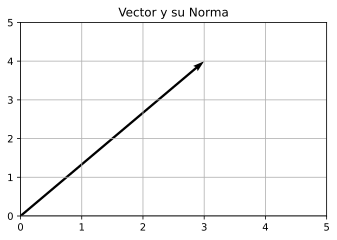
\includegraphics{presentacion_files/figure-pdf/cell-2-output-1.pdf}

\begin{center}\rule{0.5\linewidth}{0.5pt}\end{center}

\subsection{Propiedades de las Normas
(I)}\label{propiedades-de-las-normas-i}

\textbf{Propiedad 1: No negatividad}

\[
||\mathbf{v}|| \geq 0 \quad \text{y} \quad ||\mathbf{v}|| = 0 \, \text{si y sólo si} \, \mathbf{v} = 0
\]

\textbf{Propiedad 2: Homogeneidad}

\[
||c \mathbf{v}|| = |c| \cdot ||\mathbf{v}||
\]

\subsection{Propiedades de las Normas
(II)}\label{propiedades-de-las-normas-ii}

\textbf{Propiedad 3: Desigualdad triangular}

\[
||\mathbf{u} + \mathbf{v}|| \leq ||\mathbf{u}|| + ||\mathbf{v}||
\]

\begin{center}\rule{0.5\linewidth}{0.5pt}\end{center}

\begin{Shaded}
\begin{Highlighting}[]
\ImportTok{import}\NormalTok{ matplotlib.pyplot }\ImportTok{as}\NormalTok{ plt}
\ImportTok{import}\NormalTok{ numpy }\ImportTok{as}\NormalTok{ np}

\NormalTok{vector\_u }\OperatorTok{=}\NormalTok{ np.array([}\DecValTok{2}\NormalTok{, }\DecValTok{3}\NormalTok{])}
\NormalTok{vector\_v }\OperatorTok{=}\NormalTok{ np.array([}\DecValTok{3}\NormalTok{, }\DecValTok{1}\NormalTok{])}
\NormalTok{origin }\OperatorTok{=}\NormalTok{ np.array([}\DecValTok{0}\NormalTok{, }\DecValTok{0}\NormalTok{])}

\NormalTok{plt.quiver(}\OperatorTok{*}\NormalTok{origin, }\OperatorTok{*}\NormalTok{vector\_u, color}\OperatorTok{=}\StringTok{\textquotesingle{}b\textquotesingle{}}\NormalTok{, scale}\OperatorTok{=}\DecValTok{1}\NormalTok{, scale\_units}\OperatorTok{=}\StringTok{\textquotesingle{}xy\textquotesingle{}}\NormalTok{, angles}\OperatorTok{=}\StringTok{\textquotesingle{}xy\textquotesingle{}}\NormalTok{, label}\OperatorTok{=}\StringTok{\textquotesingle{}u\textquotesingle{}}\NormalTok{)}
\NormalTok{plt.quiver(}\OperatorTok{*}\NormalTok{origin, }\OperatorTok{*}\NormalTok{vector\_v, color}\OperatorTok{=}\StringTok{\textquotesingle{}r\textquotesingle{}}\NormalTok{, scale}\OperatorTok{=}\DecValTok{1}\NormalTok{, scale\_units}\OperatorTok{=}\StringTok{\textquotesingle{}xy\textquotesingle{}}\NormalTok{, angles}\OperatorTok{=}\StringTok{\textquotesingle{}xy\textquotesingle{}}\NormalTok{, label}\OperatorTok{=}\StringTok{\textquotesingle{}v\textquotesingle{}}\NormalTok{)}
\NormalTok{plt.quiver(}\OperatorTok{*}\NormalTok{origin, }\OperatorTok{*}\NormalTok{(vector\_u }\OperatorTok{+}\NormalTok{ vector\_v), color}\OperatorTok{=}\StringTok{\textquotesingle{}g\textquotesingle{}}\NormalTok{, scale}\OperatorTok{=}\DecValTok{1}\NormalTok{, scale\_units}\OperatorTok{=}\StringTok{\textquotesingle{}xy\textquotesingle{}}\NormalTok{, angles}\OperatorTok{=}\StringTok{\textquotesingle{}xy\textquotesingle{}}\NormalTok{, label}\OperatorTok{=}\StringTok{\textquotesingle{}u+v\textquotesingle{}}\NormalTok{)}

\NormalTok{plt.xlim(}\DecValTok{0}\NormalTok{, }\DecValTok{6}\NormalTok{)  }\CommentTok{\# Ajusta los límites de los ejes para que todos los vectores estén dentro de la vista}
\NormalTok{plt.ylim(}\DecValTok{0}\NormalTok{, }\DecValTok{6}\NormalTok{)}
\NormalTok{plt.axhline(}\DecValTok{0}\NormalTok{, color}\OperatorTok{=}\StringTok{\textquotesingle{}black\textquotesingle{}}\NormalTok{, linewidth}\OperatorTok{=}\FloatTok{0.5}\NormalTok{)}
\NormalTok{plt.axvline(}\DecValTok{0}\NormalTok{, color}\OperatorTok{=}\StringTok{\textquotesingle{}black\textquotesingle{}}\NormalTok{, linewidth}\OperatorTok{=}\FloatTok{0.5}\NormalTok{)}
\NormalTok{plt.title(}\StringTok{"Desigualdad Triangular"}\NormalTok{)}
\NormalTok{plt.grid(}\VariableTok{True}\NormalTok{)}
\NormalTok{plt.legend()}
\NormalTok{plt.show()}
\end{Highlighting}
\end{Shaded}

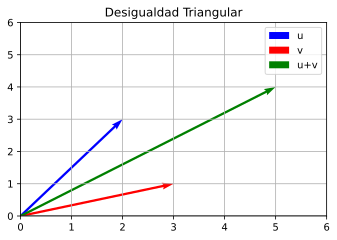
\includegraphics{presentacion_files/figure-pdf/cell-3-output-1.pdf}

\begin{center}\rule{0.5\linewidth}{0.5pt}\end{center}

\subsection{Tipos de Normas (I)}\label{tipos-de-normas-i}

Norma Euclidiana ( L\_2 ):

\[
||\mathbf{v}||_2 = \sqrt{\sum_{i=1}^n v_i^2}
\]

\subsection{Tipos de Normas (II)}\label{tipos-de-normas-ii}

Norma ( L\_1 ) (Manhattan):

\[
||\mathbf{v}||_1 = \sum_{i=1}^n |v_i|
\]

\begin{Shaded}
\begin{Highlighting}[]
\NormalTok{vector }\OperatorTok{=}\NormalTok{ np.array([}\DecValTok{3}\NormalTok{, }\DecValTok{4}\NormalTok{])}

\NormalTok{plt.plot([}\DecValTok{0}\NormalTok{, }\DecValTok{3}\NormalTok{], [}\DecValTok{0}\NormalTok{, }\DecValTok{4}\NormalTok{], label}\OperatorTok{=}\StringTok{"Norma L2"}\NormalTok{)}
\NormalTok{plt.plot([}\DecValTok{0}\NormalTok{, }\DecValTok{3}\NormalTok{], [}\DecValTok{0}\NormalTok{, }\DecValTok{0}\NormalTok{], }\StringTok{\textquotesingle{}r{-}{-}\textquotesingle{}}\NormalTok{, label}\OperatorTok{=}\StringTok{"Manhattan X"}\NormalTok{)}
\NormalTok{plt.plot([}\DecValTok{3}\NormalTok{, }\DecValTok{3}\NormalTok{], [}\DecValTok{0}\NormalTok{, }\DecValTok{4}\NormalTok{], }\StringTok{\textquotesingle{}r{-}{-}\textquotesingle{}}\NormalTok{, label}\OperatorTok{=}\StringTok{"Manhattan Y"}\NormalTok{)}
\NormalTok{plt.title(}\StringTok{"Comparación de Normas L1 y L2"}\NormalTok{)}
\NormalTok{plt.grid(}\VariableTok{True}\NormalTok{)}
\NormalTok{plt.legend()}
\NormalTok{plt.show()}
\end{Highlighting}
\end{Shaded}

\includegraphics{presentacion_files/figure-pdf/cell-4-output-1.pdf}

\subsection{\texorpdfstring{Norma \(L_\infty\) (Norma
Máxima)}{Norma L\_\textbackslash infty (Norma Máxima)}}\label{norma-l_infty-norma-muxe1xima}

\[
||\mathbf{v}||_\infty = \max_i |v_i|
\]

\subsection{Aplicaciones de las
Normas}\label{aplicaciones-de-las-normas}

Aplicaciones comunes:

\begin{itemize}
\item
  Normalización de vectores para algoritmos de aprendizaje automático.
\item
  Cálculo de distancias entre puntos en análisis de datos.
\item
  Aplicaciones en física, como la mecánica y la óptica.
\end{itemize}

\begin{center}\rule{0.5\linewidth}{0.5pt}\end{center}

\begin{Shaded}
\begin{Highlighting}[]
\ImportTok{import}\NormalTok{ matplotlib.pyplot }\ImportTok{as}\NormalTok{ plt}
\ImportTok{import}\NormalTok{ numpy }\ImportTok{as}\NormalTok{ np}

\NormalTok{vector }\OperatorTok{=}\NormalTok{ np.array([}\DecValTok{3}\NormalTok{, }\DecValTok{4}\NormalTok{])}
\NormalTok{origin }\OperatorTok{=}\NormalTok{ np.array([}\DecValTok{0}\NormalTok{, }\DecValTok{0}\NormalTok{])}

\CommentTok{\# Normalización del vector}
\NormalTok{vector\_normalizado }\OperatorTok{=}\NormalTok{ vector }\OperatorTok{/}\NormalTok{ np.linalg.norm(vector)}

\CommentTok{\# Dibujamos el vector normalizado}
\NormalTok{plt.quiver(}\OperatorTok{*}\NormalTok{origin, }\OperatorTok{*}\NormalTok{vector\_normalizado, color}\OperatorTok{=}\StringTok{\textquotesingle{}b\textquotesingle{}}\NormalTok{, scale}\OperatorTok{=}\DecValTok{1}\NormalTok{, scale\_units}\OperatorTok{=}\StringTok{\textquotesingle{}xy\textquotesingle{}}\NormalTok{, angles}\OperatorTok{=}\StringTok{\textquotesingle{}xy\textquotesingle{}}\NormalTok{, label}\OperatorTok{=}\StringTok{\textquotesingle{}Vector Normalizado\textquotesingle{}}\NormalTok{)}

\CommentTok{\# Ajustamos los límites de los ejes para que todo el vector esté en la vista}
\NormalTok{plt.xlim(}\OperatorTok{{-}}\DecValTok{1}\NormalTok{, }\DecValTok{2}\NormalTok{)  }\CommentTok{\# Los valores pueden ajustarse según sea necesario}
\NormalTok{plt.ylim(}\OperatorTok{{-}}\DecValTok{1}\NormalTok{, }\DecValTok{2}\NormalTok{)}
\NormalTok{plt.axhline(}\DecValTok{0}\NormalTok{, color}\OperatorTok{=}\StringTok{\textquotesingle{}black\textquotesingle{}}\NormalTok{, linewidth}\OperatorTok{=}\FloatTok{0.5}\NormalTok{)}
\NormalTok{plt.axvline(}\DecValTok{0}\NormalTok{, color}\OperatorTok{=}\StringTok{\textquotesingle{}black\textquotesingle{}}\NormalTok{, linewidth}\OperatorTok{=}\FloatTok{0.5}\NormalTok{)}
\NormalTok{plt.title(}\StringTok{"Normalización de un Vector"}\NormalTok{)}
\NormalTok{plt.grid(}\VariableTok{True}\NormalTok{)}
\NormalTok{plt.legend()}
\NormalTok{plt.show()}
\end{Highlighting}
\end{Shaded}

\includegraphics{presentacion_files/figure-pdf/cell-5-output-1.pdf}

\begin{center}\rule{0.5\linewidth}{0.5pt}\end{center}

\subsection{Calculo de normas}\label{calculo-de-normas}

\subsubsection{\texorpdfstring{Norma \(L_1\) (Manhattan) en
Logística}{Norma L\_1 (Manhattan) en Logística}}\label{norma-l_1-manhattan-en-loguxedstica}

\textbf{Contexto:} Un repartidor debe viajar entre dos puntos de una
ciudad que sigue una disposición en cuadrícula. La ciudad solo permite
moverse en dirección horizontal o vertical.

Dado un vector de desplazamiento \(\mathbf{d} = (3, 7)\), calcula la
norma \(L_1\) y proporciona una interpretación en términos de distancia
recorrida.

\[
||\mathbf{d}||_1 = |3| + |7| = 3 + 7 = 10
\]

\begin{center}\rule{0.5\linewidth}{0.5pt}\end{center}

\textbf{Interpretación:} La norma \(L_1\) en este contexto es la
distancia total recorrida por el repartidor, sumando los movimientos
horizontales y verticales. Representa la ``distancia de taxi'' o la
distancia efectiva en una ciudad con una cuadrícula.

\begin{center}\rule{0.5\linewidth}{0.5pt}\end{center}

\subsection{\texorpdfstring{Norma \(L_2\) (Euclidiana) en
Física}{Norma L\_2 (Euclidiana) en Física}}\label{norma-l_2-euclidiana-en-fuxedsica}

\textbf{Contexto:} En un sistema físico, la norma Euclidiana se utiliza
para calcular la magnitud de la velocidad de un objeto que se mueve en
el espacio tridimensional.

Dado el vector de velocidad \(\mathbf{v} = (2, 3, 6)\), calcula la norma
\(L_2\) y proporciona una interpretación en términos de la magnitud de
la velocidad.

\[
||\mathbf{v}||_2 = \sqrt{2^2 + 3^2 + 6^2} = \sqrt{4 + 9 + 36} = \sqrt{49} = 7
\]

\begin{center}\rule{0.5\linewidth}{0.5pt}\end{center}

\textbf{Interpretación:} La norma \(L_2\) en este contexto te dará la
magnitud de la velocidad, lo que indica la rapidez con la que el objeto
se está moviendo en el espacio. Esta magnitud es la velocidad total en
metros por segundo.

\begin{center}\rule{0.5\linewidth}{0.5pt}\end{center}

\subsubsection{\texorpdfstring{Norma \(L_\infty\) (Máxima) en Control de
Calidad}{Norma L\_\textbackslash infty (Máxima) en Control de Calidad}}\label{norma-l_infty-muxe1xima-en-control-de-calidad}

\textbf{Contexto:} En control de calidad, la norma \(L_\infty\) se
utiliza para detectar la desviación máxima de un conjunto de datos.

Dado el vector de errores de medición
\(\mathbf{e} = (-0.1, 0.05, -0.2, 0.15)\), calcula la norma \(L_\infty\)
y proporciona una interpretación en términos de la desviación máxima.

\[
||\mathbf{e}||_\infty = \max \{|-0.1|, |0.05|, |-0.2|, |0.15|\}
\] \[ = \max \{0.1, 0.05, 0.2, 0.15\} = 0.2
\]

\begin{center}\rule{0.5\linewidth}{0.5pt}\end{center}

\textbf{Interpretación:} La norma \(L_\infty\) te da la desviación más
grande en valor absoluto, lo que indica cuál es el mayor error de
medición en el conjunto de datos. Este valor es importante para evaluar
el peor caso en términos de precisión.

\begin{center}\rule{0.5\linewidth}{0.5pt}\end{center}

\subsection{\texorpdfstring{Distancia \(L_1\)
(Manhattan)}{Distancia L\_1 (Manhattan)}}\label{distancia-l_1-manhattan}

La distancia \(L_1\) entre dos puntos \(\mathbf{x} = (x_1, x_2)\) y
\(\mathbf{y} = (y_1, y_2)\) es:

\[
d_{L_1}(\mathbf{x}, \mathbf{y}) = |x_1 - y_1| + |x_2 - y_2|
\]

\begin{center}\rule{0.5\linewidth}{0.5pt}\end{center}

Esta distancia sigue caminos horizontales y verticales, como en una
cuadrícula.

\begin{Shaded}
\begin{Highlighting}[]
\ImportTok{import}\NormalTok{ numpy }\ImportTok{as}\NormalTok{ np}
\ImportTok{import}\NormalTok{ matplotlib.pyplot }\ImportTok{as}\NormalTok{ plt}

\CommentTok{\# Definir puntos}
\NormalTok{x }\OperatorTok{=}\NormalTok{ np.array([}\DecValTok{1}\NormalTok{, }\DecValTok{2}\NormalTok{])}
\NormalTok{y }\OperatorTok{=}\NormalTok{ np.array([}\DecValTok{4}\NormalTok{, }\DecValTok{6}\NormalTok{])}

\CommentTok{\# Calcular distancia L1}
\NormalTok{L1\_distance }\OperatorTok{=}\NormalTok{ np.}\BuiltInTok{sum}\NormalTok{(np.}\BuiltInTok{abs}\NormalTok{(x }\OperatorTok{{-}}\NormalTok{ y))}

\CommentTok{\# Gráfico del camino L1}
\NormalTok{plt.plot([x[}\DecValTok{0}\NormalTok{], y[}\DecValTok{0}\NormalTok{]], [x[}\DecValTok{1}\NormalTok{], x[}\DecValTok{1}\NormalTok{]], }\StringTok{\textquotesingle{}r{-}{-}\textquotesingle{}}\NormalTok{, label}\OperatorTok{=}\StringTok{"Desplazamiento Horizontal"}\NormalTok{)}
\NormalTok{plt.plot([y[}\DecValTok{0}\NormalTok{], y[}\DecValTok{0}\NormalTok{]], [x[}\DecValTok{1}\NormalTok{], y[}\DecValTok{1}\NormalTok{]], }\StringTok{\textquotesingle{}r{-}{-}\textquotesingle{}}\NormalTok{, label}\OperatorTok{=}\StringTok{"Desplazamiento Vertical"}\NormalTok{)}
\NormalTok{plt.scatter([x[}\DecValTok{0}\NormalTok{], y[}\DecValTok{0}\NormalTok{]], [x[}\DecValTok{1}\NormalTok{], y[}\DecValTok{1}\NormalTok{]], c}\OperatorTok{=}\StringTok{\textquotesingle{}b\textquotesingle{}}\NormalTok{)}
\NormalTok{plt.text(x[}\DecValTok{0}\NormalTok{], x[}\DecValTok{1}\NormalTok{], }\StringTok{\textquotesingle{}Punto A\textquotesingle{}}\NormalTok{, fontsize}\OperatorTok{=}\DecValTok{12}\NormalTok{)}
\NormalTok{plt.text(y[}\DecValTok{0}\NormalTok{], y[}\DecValTok{1}\NormalTok{], }\StringTok{\textquotesingle{}Punto B\textquotesingle{}}\NormalTok{, fontsize}\OperatorTok{=}\DecValTok{12}\NormalTok{)}
\NormalTok{plt.title(}\SpecialStringTok{f"Distancia $L\_1$: }\SpecialCharTok{\{}\NormalTok{L1\_distance}\SpecialCharTok{\}}\SpecialStringTok{"}\NormalTok{)}
\NormalTok{plt.grid(}\VariableTok{True}\NormalTok{)}
\NormalTok{plt.legend()}
\NormalTok{plt.show()}
\end{Highlighting}
\end{Shaded}

\includegraphics{presentacion_files/figure-pdf/cell-6-output-1.pdf}

\begin{center}\rule{0.5\linewidth}{0.5pt}\end{center}

\subsection{\texorpdfstring{Distancia \(L_2\)
(Euclidiana)}{Distancia L\_2 (Euclidiana)}}\label{distancia-l_2-euclidiana}

La distancia \(L_2\) entre dos puntos \(\mathbf{x} = (x_1, x_2)\) y
\(\mathbf{y} = (y_1, y_2)\) es:

\[
d_{L_2}(\mathbf{x}, \mathbf{y}) = \sqrt{(x_1 - y_1)^2 + (x_2 - y_2)^2}
\]

Esta distancia representa la línea recta más corta entre los dos puntos.

\begin{center}\rule{0.5\linewidth}{0.5pt}\end{center}

\begin{Shaded}
\begin{Highlighting}[]
\CommentTok{\# Calcular distancia L2}
\NormalTok{L2\_distance }\OperatorTok{=}\NormalTok{ np.sqrt(np.}\BuiltInTok{sum}\NormalTok{((x }\OperatorTok{{-}}\NormalTok{ y) }\OperatorTok{**} \DecValTok{2}\NormalTok{))}

\CommentTok{\# Gráfico del camino L2}
\NormalTok{plt.plot([x[}\DecValTok{0}\NormalTok{], y[}\DecValTok{0}\NormalTok{]], [x[}\DecValTok{1}\NormalTok{], y[}\DecValTok{1}\NormalTok{]], }\StringTok{\textquotesingle{}g{-}\textquotesingle{}}\NormalTok{, label}\OperatorTok{=}\StringTok{"Línea Recta"}\NormalTok{)}
\NormalTok{plt.scatter([x[}\DecValTok{0}\NormalTok{], y[}\DecValTok{0}\NormalTok{]], [x[}\DecValTok{1}\NormalTok{], y[}\DecValTok{1}\NormalTok{]], c}\OperatorTok{=}\StringTok{\textquotesingle{}b\textquotesingle{}}\NormalTok{)}
\NormalTok{plt.text(x[}\DecValTok{0}\NormalTok{], x[}\DecValTok{1}\NormalTok{], }\StringTok{\textquotesingle{}Punto A\textquotesingle{}}\NormalTok{, fontsize}\OperatorTok{=}\DecValTok{12}\NormalTok{)}
\NormalTok{plt.text(y[}\DecValTok{0}\NormalTok{], y[}\DecValTok{1}\NormalTok{], }\StringTok{\textquotesingle{}Punto B\textquotesingle{}}\NormalTok{, fontsize}\OperatorTok{=}\DecValTok{12}\NormalTok{)}
\NormalTok{plt.title(}\SpecialStringTok{f"Distancia $L\_2$: }\SpecialCharTok{\{}\NormalTok{L2\_distance}\SpecialCharTok{\}}\SpecialStringTok{"}\NormalTok{)}
\NormalTok{plt.grid(}\VariableTok{True}\NormalTok{)}
\NormalTok{plt.legend()}
\NormalTok{plt.show()}
\end{Highlighting}
\end{Shaded}

\includegraphics{presentacion_files/figure-pdf/cell-7-output-1.pdf}

\begin{center}\rule{0.5\linewidth}{0.5pt}\end{center}

\subsection{\texorpdfstring{Distancia \(L_\infty\)
(Máxima)}{Distancia L\_\textbackslash infty (Máxima)}}\label{distancia-l_infty-muxe1xima}

La distancia \(L_\infty\) entre dos puntos \(\mathbf{x} = (x_1, x_2)\) y
\(\mathbf{y} = (y_1, y_2)\) es:

\[
d_{L_\infty}(\mathbf{x}, \mathbf{y}) = \max(|x_1 - y_1|, |x_2 - y_2|)
\]

\begin{center}\rule{0.5\linewidth}{0.5pt}\end{center}

Esta distancia se enfoca en el mayor desplazamiento en cualquier
coordenada.

\begin{Shaded}
\begin{Highlighting}[]
\CommentTok{\# Calcular distancia Linf}
\NormalTok{Linf\_distance }\OperatorTok{=}\NormalTok{ np.}\BuiltInTok{max}\NormalTok{(np.}\BuiltInTok{abs}\NormalTok{(x }\OperatorTok{{-}}\NormalTok{ y))}

\CommentTok{\# Gráfico del camino Linf}
\NormalTok{plt.plot([x[}\DecValTok{0}\NormalTok{], y[}\DecValTok{0}\NormalTok{]], [x[}\DecValTok{1}\NormalTok{], x[}\DecValTok{1}\NormalTok{]], }\StringTok{\textquotesingle{}r{-}{-}\textquotesingle{}}\NormalTok{, label}\OperatorTok{=}\StringTok{"Desplazamiento Horizontal"}\NormalTok{)}
\NormalTok{plt.plot([y[}\DecValTok{0}\NormalTok{], y[}\DecValTok{0}\NormalTok{]], [x[}\DecValTok{1}\NormalTok{], y[}\DecValTok{1}\NormalTok{]], }\StringTok{\textquotesingle{}r{-}{-}\textquotesingle{}}\NormalTok{, label}\OperatorTok{=}\StringTok{"Desplazamiento Vertical"}\NormalTok{)}
\NormalTok{plt.scatter([x[}\DecValTok{0}\NormalTok{], y[}\DecValTok{0}\NormalTok{]], [x[}\DecValTok{1}\NormalTok{], y[}\DecValTok{1}\NormalTok{]], c}\OperatorTok{=}\StringTok{\textquotesingle{}b\textquotesingle{}}\NormalTok{)}
\NormalTok{plt.text(x[}\DecValTok{0}\NormalTok{], x[}\DecValTok{1}\NormalTok{], }\StringTok{\textquotesingle{}Punto A\textquotesingle{}}\NormalTok{, fontsize}\OperatorTok{=}\DecValTok{12}\NormalTok{)}
\NormalTok{plt.text(y[}\DecValTok{0}\NormalTok{], y[}\DecValTok{1}\NormalTok{], }\StringTok{\textquotesingle{}Punto B\textquotesingle{}}\NormalTok{, fontsize}\OperatorTok{=}\DecValTok{12}\NormalTok{)}
\NormalTok{plt.title(}\SpecialStringTok{f"Distancia $L\_\textbackslash{}infty$: }\SpecialCharTok{\{}\NormalTok{Linf\_distance}\SpecialCharTok{\}}\SpecialStringTok{"}\NormalTok{)}
\NormalTok{plt.grid(}\VariableTok{True}\NormalTok{)}
\NormalTok{plt.legend()}
\NormalTok{plt.show()}
\end{Highlighting}
\end{Shaded}

\begin{verbatim}
<>:10: SyntaxWarning: invalid escape sequence '\i'
<>:10: SyntaxWarning: invalid escape sequence '\i'
/tmp/ipykernel_20817/1327578443.py:10: SyntaxWarning: invalid escape sequence '\i'
  plt.title(f"Distancia $L_\infty$: {Linf_distance}")
\end{verbatim}

\includegraphics{presentacion_files/figure-pdf/cell-8-output-2.pdf}

\begin{center}\rule{0.5\linewidth}{0.5pt}\end{center}

\subsection{Comparación de las
distancias}\label{comparaciuxf3n-de-las-distancias}

Podemos comparar las tres distancias calculadas entre los puntos \(A\) y
\(B\):

\begin{itemize}
\tightlist
\item
  Distancia \(L_1\): \(|x_1 - y_1| + |x_2 - y_2|\)
\item
  Distancia \(L_2\): \(\sqrt{(x_1 - y_1)^2 + (x_2 - y_2)^2}\)
\item
  Distancia \(L_\infty\): \(\max(|x_1 - y_1|, |x_2 - y_2|)\)
\end{itemize}

Cada norma mide la distancia de una forma diferente. La distancia
\(L_1\) suma las diferencias en las coordenadas, la distancia \(L_2\)
mide la línea recta más corta, y la distancia \(L_\infty\) se enfoca en
el mayor desplazamiento.

\subsection{Como te imaginas que seria una circunferencia en las
diferentes
distancias?}\label{como-te-imaginas-que-seria-una-circunferencia-en-las-diferentes-distancias}

\textbf{Definicio de circunferencia} Una circunferencia es el lugar
geométrico de los puntos del plano cuya distancia a otro punto fijo,
llamado centro, es constante.

\begin{center}\rule{0.5\linewidth}{0.5pt}\end{center}

\begin{Shaded}
\begin{Highlighting}[]
\NormalTok{plt.figure(figsize}\OperatorTok{=}\NormalTok{(}\DecValTok{6}\NormalTok{, }\DecValTok{6}\NormalTok{))}

\CommentTok{\# Rango de ángulos para dibujar las "circunferencias"}
\NormalTok{theta }\OperatorTok{=}\NormalTok{ np.linspace(}\DecValTok{0}\NormalTok{, }\DecValTok{2} \OperatorTok{*}\NormalTok{ np.pi, }\DecValTok{100}\NormalTok{)}

\CommentTok{\# Función para dibujar circunferencia bajo norma L1}
\NormalTok{x\_L1 }\OperatorTok{=}\NormalTok{ np.}\BuiltInTok{abs}\NormalTok{(np.cos(theta)) }\OperatorTok{+}\NormalTok{ np.}\BuiltInTok{abs}\NormalTok{(np.sin(theta))  }\CommentTok{\# L1 suma de valores absolutos}
\NormalTok{x1 }\OperatorTok{=}\NormalTok{ np.cos(theta) }\OperatorTok{/}\NormalTok{ x\_L1}
\NormalTok{y1 }\OperatorTok{=}\NormalTok{ np.sin(theta) }\OperatorTok{/}\NormalTok{ x\_L1}

\CommentTok{\# Función para dibujar circunferencia bajo norma L2}
\NormalTok{x2 }\OperatorTok{=}\NormalTok{ np.cos(theta)}
\NormalTok{y2 }\OperatorTok{=}\NormalTok{ np.sin(theta)}

\CommentTok{\# Dibujar un cuadrado para la norma L\_inf (Máxima)}
\NormalTok{x3 }\OperatorTok{=}\NormalTok{ np.array([}\OperatorTok{{-}}\DecValTok{1}\NormalTok{, }\DecValTok{1}\NormalTok{, }\DecValTok{1}\NormalTok{, }\OperatorTok{{-}}\DecValTok{1}\NormalTok{, }\OperatorTok{{-}}\DecValTok{1}\NormalTok{])}
\NormalTok{y3 }\OperatorTok{=}\NormalTok{ np.array([}\OperatorTok{{-}}\DecValTok{1}\NormalTok{, }\OperatorTok{{-}}\DecValTok{1}\NormalTok{, }\DecValTok{1}\NormalTok{, }\DecValTok{1}\NormalTok{, }\OperatorTok{{-}}\DecValTok{1}\NormalTok{])}

\CommentTok{\# Dibujar las tres circunferencias en el mismo plano cartesiano}
\NormalTok{plt.plot(x1, y1, label}\OperatorTok{=}\StringTok{\textquotesingle{}$L\_1$\textquotesingle{}}\NormalTok{, color}\OperatorTok{=}\StringTok{\textquotesingle{}r\textquotesingle{}}\NormalTok{)}
\NormalTok{plt.plot(x2, y2, label}\OperatorTok{=}\StringTok{\textquotesingle{}$L\_2$\textquotesingle{}}\NormalTok{, color}\OperatorTok{=}\StringTok{\textquotesingle{}g\textquotesingle{}}\NormalTok{)}
\NormalTok{plt.plot(x3, y3, label}\OperatorTok{=}\StringTok{\textquotesingle{}$L\_\textbackslash{}infty$\textquotesingle{}}\NormalTok{, color}\OperatorTok{=}\StringTok{\textquotesingle{}b\textquotesingle{}}\NormalTok{)}

\CommentTok{\# Configuraciones del gráfico}
\NormalTok{plt.gca().set\_aspect(}\StringTok{\textquotesingle{}equal\textquotesingle{}}\NormalTok{)}
\NormalTok{plt.title(}\StringTok{\textquotesingle{}Comparación de normas $L\_1$, $L\_2$ y $L\_\textbackslash{}infty$\textquotesingle{}}\NormalTok{)}
\NormalTok{plt.grid(}\VariableTok{True}\NormalTok{)}
\NormalTok{plt.legend()}
\NormalTok{plt.xlim([}\OperatorTok{{-}}\FloatTok{1.5}\NormalTok{, }\FloatTok{1.5}\NormalTok{])}
\NormalTok{plt.ylim([}\OperatorTok{{-}}\FloatTok{1.5}\NormalTok{, }\FloatTok{1.5}\NormalTok{])}

\CommentTok{\# Mostrar la figura}
\NormalTok{plt.show()}
\end{Highlighting}
\end{Shaded}

\begin{verbatim}
<>:22: SyntaxWarning: invalid escape sequence '\i'
<>:26: SyntaxWarning: invalid escape sequence '\i'
<>:22: SyntaxWarning: invalid escape sequence '\i'
<>:26: SyntaxWarning: invalid escape sequence '\i'
/tmp/ipykernel_20817/1189076720.py:22: SyntaxWarning: invalid escape sequence '\i'
  plt.plot(x3, y3, label='$L_\infty$', color='b')
/tmp/ipykernel_20817/1189076720.py:26: SyntaxWarning: invalid escape sequence '\i'
  plt.title('Comparación de normas $L_1$, $L_2$ y $L_\infty$')
\end{verbatim}

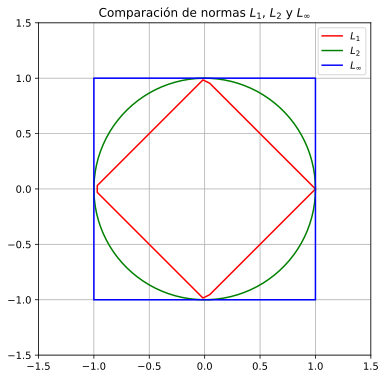
\includegraphics{presentacion_files/figure-pdf/cell-9-output-2.pdf}




\end{document}
